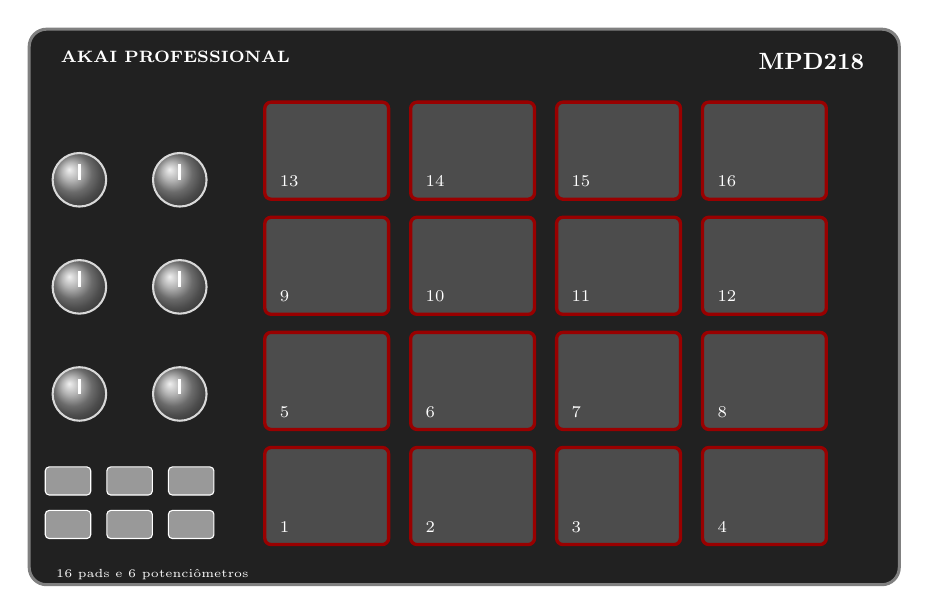
\begin{tikzpicture}[x=1cm,y=1cm,scale=0.85,every node/.style={transform shape}]
\draw[rounded corners=0.22cm,fill=black!87,draw=black!50,line width=1.1pt] (0,0) rectangle (13,8.3);
\node[anchor=west,text=white,font=\bfseries\scriptsize] at (0.35,7.88) {AKAI PROFESSIONAL};
\node[anchor=east,text=white,font=\bfseries] at (12.6,7.82) {MPD218};
\foreach \y in {2.85,4.45,6.05}{
 \foreach \x in {0.75,2.25}{
  \shade[ball color=black!40] (\x,\y) circle (0.39);
  \draw[draw=black!15,line width=0.75pt] (\x,\y) circle (0.40);
  \draw[draw=white!70,line width=1pt] (\x,\y) -- ++(0,0.23);
 }
}
\foreach \i in {0,1,2,3}{
 \foreach \j in {0,1,2,3}{
  \pgfmathtruncatemacro{\padnum}{4*\i+\j+1}
  \draw[fill=black!70,draw=red!60!black,line width=1.2pt,rounded corners=0.08cm]
    (3.52+2.18*\j,0.60+1.72*\i) rectangle (5.37+2.18*\j,2.05+1.72*\i);
  \node[anchor=south west,text=white,font=\scriptsize] at (3.62+2.18*\j,0.66+1.72*\i) {\padnum};
 }
}
\foreach \y in {0.90,1.55}{
 \foreach \x in {0.58,1.50,2.42}{
  \draw[fill=black!40,draw=white!50,rounded corners=0.05cm]
    (\x-0.34,\y-0.21) rectangle (\x+0.34,\y+0.21);
 }
}
\node[text=white,font=\tiny,align=left,anchor=west] at (0.28,0.15) {16 pads e 6 potenciômetros};
\end{tikzpicture}
